\part{Richiami di termodinamica}
\begin{adjustwidth}{2in}{}
	In questo modulo ci si concentrerà sullo studio dell'impianto per la generazione di energia e non più sulla macchina. \newline
	
	Ci si occuperà di impianti che trattano i due fluidi più disponibili in natura: aria per mezzo degli impianti a gas, e acqua attraverso gli impianti a vapore. \newline
	
	Un componente di un impianto viene progettato per effettuare scambio di calore o scambio di lavoro, questo perché  avere un sistema che riesca a scambiare sia calore che lavoro, è praticamente irrealizzabile: per scambiare calore si necessitano di grandi superfici di contatto, condizione che non è possibile ritrovare nelle palette di una turbina. L'unico sistema in grado di scambiare sia calore che lavoro è il motore a combustione interna, dove nello stesso cilindro si svolge sia la combustione - che produce calore - sia l'espansione del gas - che scambia lavoro -. \newline
	
	In questo corso ci si occuperà solamente di sistemi ad aria o ad acqua in cui si compiranno separatamente scambi di calore e lavoro. 
	
	I sistemi che si studieranno sono detti "\textit{in permanenza}": la variazione nel tempo delle grandezze fisiche risulta trascurabile, tutti i fenomeni che si andranno ad analizzare saranno relativi a sistemi che non mutano nel tempo, senza transitori. \newline 
	
	In condizioni "di permanenza" si può così individuare un certo "\textit{stato fisico}", questo è un insieme di condizioni fisiche nel quale si trova il fluido in oggetto, uno stato fisico è caratterizzabile solamente attraverso i sensi e quindi tramite delle grandezze misurabili come $V, P, T$; il volume può essere visto sia in maniera estensiva, e quindi misurandolo in $m^3$, oppure può essere svincolato dalla massa ed essere reso intensivo, considerandolo specifico $v$ e misurandolo in $\nicefrac{m^3}{kg}$, se si è in grado di stabilire tali grandezze allora si può caratterizzare lo stato fisico. \newline
	
	Rimane ovviamente possibile per una sostanza in un certo stato fisico subire una variazione a seguito di un'alterazione delle condizioni ambientali: è possibile cioè passare da uno stato fisico all'altro modificando o pressione o temperatura o il volume a disposizione. \newline
	
	
	Per caratterizzare completamente un certo stato fisico è sempre necessario conoscere tutte e tre le grandezze fisiche fondamentali? \newline
	
	\section{Regola di Gibbs - Helmoltz o legge della varianza}
	La varianza $\nu$ è pari a 
	\begin{equation}\label{eq:1.0}
		\boxed{\nu = N-X+2}
	\end{equation}
	Dove $N$ è il numero di componenti indipendenti ed $X$ è il numero di fasi. \newline
	
	La materia si può presentare in 4 fasi, solida gassosa, liquida, plasma. 
	
	Per l'aria, pur essendo una miscela di gas in cui è presente un certo titolo di vapore, si può assumere senza troppe perdite di generalità, $X=N=1$, questo perché dalla psicometria, anche avendo un componente ed una fase, è possibile risalire a ciò che manca. 
	
	La varianza dell'aria sarà in questo modo pari a 2, significa che sono necessarie soltanto due informazioni tra $V,P,T$ per stabilire  la terza e avere interamente caratterizzato lo stato fisico. \newline
	
	Diverso è il discorso per un sistema acqua-vapore, in questo caso il numero di componenti indipendenti è uno: acqua, ma è il numero di fasi a cambiare, diviene infatti pari a due
	\[\nu = 1-2+2 = 1\] 
	Essendo la varianza pari a 1, basta una sola grandezza sensibile per caratterizzare completamente lo stato  fisico. 
	
	Infatti è più che noto che ad una determinata pressione di saturazione, corrisponde automaticamente una determinata temperatura di saturazione. \newline
	
	Nel caso invece di vapore surriscaldato sussiste sempre lo stesso unico componente, ma stavolta in una sola fase, quella di vapore, per cui
	\[\nu = 1-1+2 = 2\] 
	E la varianza torna ad essere 2. \newline
	
	Esiste anche una particolare condizione,  quella di punto triplo nota a priori, in cui la varianza è nulla, perché ad un solo componente corrispondono 3 fasi. Per l'acqua corrisponde a $T = 0.0075\degree C$ e $P = 0.6117 kPa$. \newline
	
	\section{Equazione di stato dei gas perfetti}
	Avere per l'aria una varianza pari a due significa che dovrà esistere un'equazione che leghi le tre grandezze sensibili in modo che, conoscendone due, diviene possibile ricavare la terza. Questa relazione viene fornita attraverso l'equazione di stato dei gas perfetti (valida per gas reali lontano dalle condizioni critiche di P e T)
	\begin{equation} \label{eq:1.1}
		\boxed{PV=nRT \qquad \textbf{R} = 8.314 \dfrac{J}{Kmol}}
	\end{equation} 
	Oppure esprimendola in termini specifici
	\[\dfrac{P}{\rho} = RT \qquad R = \dfrac{\textbf{R}}{\text{Massa Molare}} \]
	L'equazione di stato rimane tuttavia una rappresentazione matematica della realtà e pertanto porterà con se delle imprecisioni, questa infatti risulterà esatta soltanto per i gas perfetti.
	
	Si introduce allora il fattore $z$ di comprimibilità, questo misurerà il rapporto 
	\[z = \dfrac{P}{\rho RT} \]
	Tanto questo rapporto si avvicina all'unità, tanto sarà possibile applicare l'equazione dei gas di stato senza perdite di generalità.
	
	Solitamente per i gas reali tale fattore è maggiore di uno, e questo significa che l'equazione di stato non rappresenta esattamente le caratteristiche del gas, tuttavia, rimanendo all'interno di uno scostamento dell'1\%, si accetta come approssimazione ingegneristica. 
	
	Tale approssimazione, nel corso di questo modulo, varrà negli impianti turbina a gas in cui la temperatura dell'aria varia tra quella ambiente e i 1500 gradi centigradi, tale approssimazione risulterà invece irrealizzabile per l'acqua, per la quale si utilizzeranno le tabelle del vapore, queste ricavate sperimentalmente. 

\newpage
	
	\section{Termodinamica}
	Per realizzare i sistemi energetici oggetto del corso ci si baserà sulla termodinamica, questa a sua volta si basa su tre principi fondamentali. 
	
	\begin{itemize}
		\item \textbf{Principio di conservazione}
		\item \textbf{Principio di equivalenza}
		\item \textbf{Principio ci evoluzione}
	\end{itemize}
	
	\subsection{Principio di conservazione}
	\begin{en}
		L'energia di un sistema rimane costante, al massimo possono cambiare i sui contributi.
	\end{en}
	\[E=mc^2 + {1\over2}mv^2 + {3\over8}\dfrac{mu^4}{c^2} + {5\over16}\dfrac{mu^6}{c^4} + \dots\]
	 
	
	\subsection{Principio di equivalenza}
	\textit{Primo principio della termodinamica per sistemi chiusi}
	
	Considerando quantità specifiche 
	\begin{equation}\label{eq:1.2}
		\boxed{\Delta u = q+\bar{l}}
	\end{equation}
	\textit{Calore e lavoro contribuiscono entrambi all'energia interna}.
	
	L'energia interna $u$ si può dividere in due categorie:
	\begin{itemize}
		\item \textbf{microscopica}, derivante dal moto vibrazionale delle molecole e misurata attraverso la temperatura
		\item \textbf{macroscopiche}, fornite dalla velocità e dalla quota
	\end{itemize}
	Si consideri in prima istanza un gas a bassa densità, caratterizzato da differenze di quota e velocità non rilevanti, in questo modo l'unico contributo di energia interna è dovuto solamente alla temperatura.
	
	
	\subsubsection{Principio di equivalenza per un sistema chiuso}
	Si assuma un contenitore indeformabile che non possa scambiare lavoro con l'esterno (questo essendo il prodotto di una forza per uno spostamento, se il contenitore  è indeformabile, non può sussistere alcun tipo di spostamento).
	
	\vspace{0.5cm}
	
	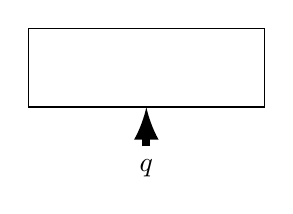
\begin{tikzpicture}[>=latex]
		\draw (2,1) rectangle (5,2);
		\draw [line width=3pt, ->] (3.5,0.5) -- (3.5,1) node [pos=0, below] {$q$};
	\end{tikzpicture}
	
	E quindi 
	\[\Delta u = q\]
	La variazione di energia interna è così dovuta solamente al calore immesso,
	nello specifico, avendo uno volume indeformabile, la trasformazione è isovolumica (isocora) quindi se si andrà ad inserire calore, si avrà giocoforza un aumento di pressione e temperatura, componenti dell'energia interna microscopica. 
	
	\newpage
	
	Se ora il contenitore viene messo in comunicazione con l'ambiente esterno tramite un pistone allora può scambiare lavoro 
	
	\vspace{0.5cm}
	
	\begin{tikzpicture}[>=latex]
		%\draw [help lines] (0,0) grid (15,15);
		\draw (2,1) -- (2,4) --  (3,4) -- (3,3) -- (5,3) -- (5,2) -- (3,2) -- (3,1) -- (2,1) -- cycle;
		\draw [pattern=north east lines] (4.5,2.05) rectangle (5,2.95);
		\draw (5,2.5) -- (5.5,2.5);
		\draw [->] (3,3.5) -- (6.5,3.5) node [pos=1, right] {$x$};
		\draw (4,3.4) -- (4,3.6);
		\draw (4.5,3.4) -- (4.5,3.6);
		\node at (4.25, 4) {dx};
		\draw [line width=3pt, ->] (6,2.5) -- (5.5,2.5) node [pos=0, right] {$l$};
		\draw [line width=3pt, ->] (1.5,2.5) -- (2,2.5) node [pos=0, left] {$q$};
	\end{tikzpicture}
	
	Se il calore fornito è nullo la trasformazione è adiabatica, allora si avrà 
	\[\Delta u = \bar{l}\]	
	
	Nel caso generale, se in un sistema avviene sia uno scambio di calore che di lavoro, a quelle già citate si aggiungeranno trasformazioni a pressione costante e a temperatura costante, ovvero, trasformazioni isobare e isoterme.
	
	Si trascuri per il  momento la presenza degli attriti, si può allora ricavare l'espressione analitica del lavoro come
	\[d\bar{l} = -Fdx \qquad F=PS \Rightarrow d\bar{l} = -PSdx = -PdV\]
	Per ottenere il lavoro
	\begin{equation} \label{eq:1.3}
		\boxed{\int d\bar{l} = \int-PdV}
	\end{equation}
	Perciò, a meno che la trasformazione non sia isobara, si dovrà conoscere la legge di variazione della pressione lungo la trasformazione. 
	
	DISEGNO diagramma pv , individuo due stati fisici e li connetto alle trasformazioni  con due curve generiche e individuo aree sottese
	
	Integrando sul diagramma $PV$ la legge di variazione della pressione si ottiene l'area sottesa alla trasformazione e quindi il lavoro. 
	
	Il lavoro si configura così come una funzione dipendente dal percorso effettuato e non dagli stati estremali del percorso: il lavoro non è una funzione di stato, non è un differenziale esatto. \newline
	
	Generalmente si scrive  
	\[du = \delta q +\delta l\]
	Perché il lavoro, non essendo un differenziale esatto, non è una funzione di stato, tuttavia l'energia interna dipende dai soli stati iniziali e finali del sistema e quindi è un differenziale esatto.
	
	L'unico modo per cui $u$ sia una differenziale esatto a partire da un differenziale non esatto è sommargli un differenziale non esatto: $q$ è un differenziale non esatto, dipende anch'esso dal percorso della trasformazione. \newline
	
	In più, poiché la densità è pari all'inverso del volume specifico
	\[\rho = \dfrac{1}{v}\]
	\[\ln\rho = -\ln v\]
	Differenziando
	\[\dfrac{d\rho}{\rho} = \dfrac{dv}{v}\]
	\[dv = -v\dfrac{d\rho}{\rho} = -\dfrac{d\rho}{\rho^2}\]
	E quindi
	\begin{equation}\label{eq:1.4}
		\boxed{dl = -PdV = P\dfrac{d\rho}{\rho^2}}
	\end{equation}
	
	\subsubsection{Principio di equivalenza per un sistema aperto}
	Ora diviene possibile scambiare massa con l'ambiente esterno 
	
	\vspace{0.5cm}
	
	\begin{tikzpicture}[>=latex]
	\draw (2,1) -- (2,4) --  (3,4) -- (3,3) -- (5,3) -- (5,2) -- (3,2) -- (3,1) -- (2,1) -- cycle;
	\draw [pattern=north east lines] (4.5,2.05) rectangle (5,2.95);
	\draw (5,3.4) -- (5,3.6);
	\draw (4.5,3.4) -- (4.5,3.6);
	\node at (4.75, 3.5) {dv};
	\draw [line width=3pt, ->] (6,2.5) -- (5,2.5) node [pos=0, right] {$dm$};
	\draw [line width=3pt, ->] (1.5,2.5) -- (2,2.5) node [pos=0, left] {$q$};
	\end{tikzpicture}
	
	Trascurando lo scambio di calore (non fornisce alcuna indicazione aggiuntiva) la massa porterà con sé la sua energia interna e una volta introdotta nel sistema e la aggiungerà a quella preesistente, in più per il trasporto della massa bisognerà esercitare un certo lavoro atto a superare la pressione intera al serbatoio, si avrà allora che l'energia interna totale diviene pari a
	\[dU = dmu_m + \underbrace{PdV}_{l_P}\]
	In cui $l_P$ è il lavoro di pulsione.
	
	Allora 
	\[dU = dm\left[u_m+P\dfrac{dv}{dm}\right] = dm\underbrace{\left[u_m+\dfrac{P}{\rho}\right]}_{h}\]
	Si individua così la funzione di stato entalpia $h$
	\begin{equation}\label{eq:1.5}
		\boxed{h = u + \dfrac{P}{\rho}}
	\end{equation}
	In questo modo si può scrivere, per un sistema aperto
	\[dU = hdm\]
	\textbf{NB}: l'entalpia è un differenziale esatto perché è composta da differenziali esatti come l'energia interna, la pressione e la densità. \newline
	
	\textbf{Come rapportare entalpia, calore e lavoro?}
	
	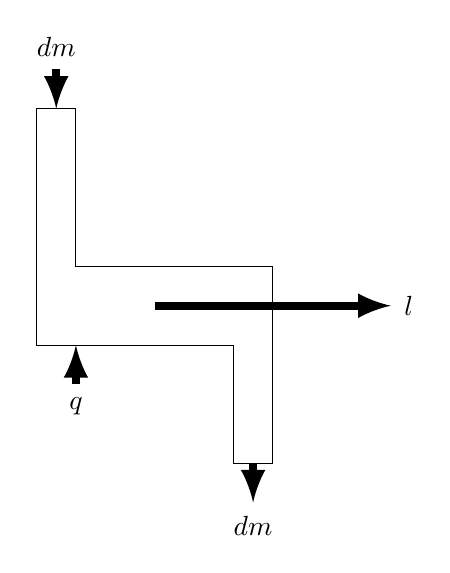
\begin{tikzpicture}[>=latex]
		\draw (2,1) -- (2,4) --  (2.5,4) -- (2.5,2) -- (5,2) -- (5,-0.5) -- (4.5,-0.5) -- (4.5,1) -- (2,1) -- cycle;
		\draw [line width=3pt, ->] (2.25,4.5) -- (2.25,4) node [pos=0, above] {$dm$};
		\draw [line width=3pt, ->] (4.75,-0.5) -- (4.75,-1) node [pos=1, below] {$dm$};
		\draw [line width=3pt, ->] (2.5,0.5) -- (2.5,1) node [pos=0, below] {$q$};
		\draw [line width=3pt, ->] (3.5,1.5) -- (6.5,1.5) node [pos=1, right] {$l$};
	\end{tikzpicture}
	
	All'interno del serbatoio un organo è capace di compiere lavoro mentre al sistema viene fornito calore, allora l'energia interna totale si potrà scrivere come
	\[dU = h_1dm_1 - h_2dm_2 + dQ+dL\]
	Se il sistema è a massa costante, ovvero tanta massa entra quanta massa esce, allora 
	\[dm_1=dm_2\]
	e quindi
	\[dU = dm(h_1 - h_2) + dQ+dL\]
	Assumendo $\Delta U=0$ quindi l'instaurarsi di un regime di funzionamento "permanente", allora varrà, ritornando a grandezze specifiche
	\[h_2 - h_1 = dq+dl\]
	Individuando l'espressione del primo principio della termodinamica per sistemi aperti
	\begin{equation} \label{eq:1.6}
		\boxed{\Delta h = dq+dl}
	\end{equation}
	
	\vspace{0.5cm}
	
	In conclusione, attraverso il principio di equivalenza, si sono individuate le espressioni del
	\begin{itemize}
		\item \textbf{Primo Principio della termodinamica per i sistemi chiusi}
		\[du = dq + d\bar{l}\]
		\item \textbf{Primo principio della termodinamica per i sistemi aperti}
		\[dh = dq+dl\]
	\end{itemize}
	E si riferiscono entrambe a due tipologie di applicazioni diverse. 
	
	La prima equazione, riconducibile ai sistemi chiusi, vede il sistema in  ottica euleriana: Si fissa un volume che viene costantemente monitorato al variare del tempo.
	
	La seconda equazione invece, riconducibile ai sistemi aperti, vede il sistema  in ottica lagrangiana: è come se si seguisse una particella di fluido dal momento in cui entra al momento in cui esce dal sistema.
	
	\subsubsection{Calori specifici}
	
	All'interno di un sistema isometrico, a volume fissato, vale
	\[d\bar{l} = 0\Rightarrow dq = du \] 
	Esiste una grandezza, il calore specifico, pari a 
	\[c = \dfrac{dq}{dT} \rightarrow dq = cdT\]
	Poiché si è detto che $q$ dipende dal percorso, allora anche $c$ dipenderà dal percorso e a volume costante si potrà individuare il calore specifico a volume costante 
	\begin{equation}\label{eq:1.7}
		\boxed{c_V = \dfrac{du}{dT} \rightarrow du = c_VdT}
	\end{equation}
		
	Analogamente, in un processo isobaro dove la pressione si mantiene costante, si avrà 
	\[dl = 0\Rightarrow dq = dh \] 
	E quindi il calore specifico a pressione costante sarà
	\begin{equation}\label{eq:1.8}
		\boxed{c_P = \dfrac{dh}{dT} \rightarrow dh = c_PdT}
	\end{equation}
	
	Spesso si incontrerà il parametro $k$, rapporto tra i due calori specifici
	\begin{equation} \label{eq:1.9}
		\boxed{k = \dfrac{c_P}{c_V}}
	\end{equation}
	
	In più, poiché è noto che 
	\[h = u + \dfrac{P}{\rho}\]
	Allora giocoforza $h>u$, siccome $c_P\propto h$ e $c_V\propto du$ allora 
	\[c_P>c_V \rightarrow k>1\]
	
	Per un processo adiabatico si può scrivere 
	\[dl=dh = du + \dfrac{P}{\rho} = du + \dfrac{dP}{\rho} - P\dfrac{d\rho}{\rho^2}\]
	Allora 
	\[dl = P\dfrac{d\rho}{\rho^2} + \dfrac{dP}{\rho} - P\dfrac{d\rho}{\rho^2} = \dfrac{dP}{\rho}\]
	
	Per cui in sostanza, se il lavoro per i sistemi chiusi si può scrivere come $\bar{l}=Pdv$, per i sistemi aperti varrà
	\begin{equation}\label{eq:1.10}
		\boxed{l = \dfrac{dP}{\rho} = vdP}
	\end{equation}
	
	E se la variazione di energia interna diventasse dipendente anche dalle componenti macroscopiche per prima erano state trascurate? 
	
	Allora per un sistema chiuso varrà che la somma delle energie in gioco dovrà essere sempre uguale alla somma di calore e lavoro
	\[dU + dE_P + dE_C = Q+\bar{L}\]
	E similmente varrà per un sistema aperto
	\[dH + dE_P + dE_C = Q+L\]
	
	
	\textbf{Per i liquidi} ad esempio se non intervengono scambi di calore $q=0$ allora varrà $du = 0$ in virtù della loro incomprimibilità e allora si ottiene 
	\[\Delta H = \cancel{\Delta U} +  \dfrac{\Delta P}{\rho} \Rightarrow L = \dfrac{\Delta P}{\rho} +\Delta E_P + \Delta E_C \]
	Se anche il lavoro è nullo, ad esempio in un sistema chiuso come può essere un condotto statorico, allora 
	\[\dfrac{\Delta P}{\rho} +\Delta E_P + \Delta E_C = 0 \]
	E quindi
	\[\dfrac{\Delta P}{\rho} +g\Delta h + {1\over2}mv^2 = 0\]
	E si ritorna all'equazione di Bernoulli. \newline
	
	\textbf{Per i gas} invece, essendo la densità piuttosto ridotta, si può scrivere 
	\[dH + \cancel{dE_P}+ dE_C = Q+L\]
	Trascurando il termine di energia potenziale. 
	
	Allora, in termini differenziali e specifici si può scrivere
	\[\underbrace{dh +  cdc}_{dh_T} = dq+dl\]
	Individuando l'entalpia totale o di ristagno $h_T$, ovvero un'entalpia che considera anche i termini cinetici
	\[h_t = h + \dfrac{c^2}{2}\]
	
	\subsection{Principio di evoluzione}
	Il principio di evoluzione sancisce che la natura si dirige sempre verso degli stati più probabili: lasciando raffreddare una bevanda calda in un ambiente ampio a temperatura inferiore, non succederà mai che la tazzina continui a riscaldarsi e l'ambiente inizi a raffreddarsi, bensì il contrario, infatti si assisterà sempre allo spontaneo raffreddamento della tazzina. 
	
	Quanto osservato empiricamente trova conferma teorica nel Secondo principio della termodinamica, questo consta di due enunciati. 
	
	\begin{itemize}
		\item \textbf{Enunciato di Clausius}
		\begin{en}
			Il calore passa spontaneamente da corpi più caldi a corpi più freddi, richiedendo per il passaggio inverso un'azione compensatrice.
		\end{en} 		
		In questo enunciato  è insito il concetto di degradazione dell'energia a seguito di uno scambio di calore, infatti se si può scambiare calore soltanto da un corpo più caldo ad un corpo più freddo allora una volta completato lo scambio non si potrà più tornare indietro. 
		
		Il concetto di "\textit{exergia}" indica il contenuto di energia termica  opportunamente scalato di un fattore correttivo che dipende dalla temperatura:  più sarà alta la temperatura, più sarà alta l'exergia. 
		
		\item \textbf{Enunciato di Clausius}\\
		\begin{en}
			Sono necessarie almeno due sorgenti termiche (di adduzione e di sottrazione) per la produzione continuativa di lavoro utile, con un sistema fluido operante ciclicamente.
		\end{en}		
	\end{itemize}
	
	Nella realtà questi enunciati sono equivalenti ({\footnotesize Equivalenza tra i principi di Kelvin e Clausius} \ref{par:eq}). \newline
	
	Un processo ciclico è un processo costituito da una serie di trasformazioni termodinamiche che riconducono periodicamente il fluido alle condizioni iniziali.
	
	\newpage
	
	Si supponga di monitorare l'energia interna, nota variabile di stato, attraverso questo impianto
	
	\vspace{0.5cm}
	
	\begin{tikzpicture}[>=latex]
		%\draw [help lines] (0,0) grid (15,15);
		% Generatore di Vapore con economizzatore
		\draw (2,9) rectangle (4,11);
		\draw [pattern=vertical lines] (2,8) rectangle (4,9);
		% Surriscaldatore e collegamento turbina
		\draw (3,11) -- (3,11.5) -- (3.5,12) -- (2.5,12.5) -- (3,13) -- (3,14) -- (9,14) -- (9,11);
		% Turbina
		\draw (9,11) -- (10,12) -- (10,9) -- (9,10) -- (9,11) -- cycle;
		\draw [line width=3pt] (10, 10.5) -- (11, 10.5);
		\node [draw, circle] at (11.35, 10.5) {$\sim$};
		\draw (10,9) -- (10,8);
		% Condensatore
		\draw (10,7.5) circle (0.5cm);
		\draw (11,8) -- (10,7.5) -- (11,7);
		\draw (10,7) -- (10,5.5);
		% Pompa di estrazione del condensato
		\draw (10,5) circle (0.5cm);
		\draw (10,4.5) -- (9.60,5.25) -- (10.40,5.25) -- cycle;
		\draw [->] (10,4.5) -- (10,2);
		% Serbatoio
		\draw (11,2) -- (11,1) -- (8,1) -- (8,2);
		\draw (11, 1.5) -- (8,1.5); 
		\draw (8,1) -- (6,1);
		% Pompa di Alimento
		\draw (5.5,1) circle (0.5cm);
		\draw (5,1) -- (5.75,1.4) -- (5.75,0.60) -- cycle;
		\draw [->] (5,1) -- (3,1) -- (3,8);
		% NOMI
		\node at (3,10) {GV}; 
		\node at (2,12) {SH};
		\node at (9.5,10.5) {T};
		\node at (11,7.5) {C};
		\node at (11, 5) {Pe};
		\node at (9.5, 0) {Serbatoio $H_2O$};
		\node at (5.5, 0) {Pa};
	\end{tikzpicture}
	
	In questa tipologia di impianto, attraverso una sorgente termica, si scalda l'acqua al fine di ottenere vapore surriscaldato ad alta pressione che una volta convogliato in turbina de permette l'estrazione del lavoro.
	
	Se come riferimento si prende il punto in ingresso al generatore di vapore (GV), allora si nota subito che in questo sistema, per ogni ciclo di funzionamento, periodicamente si ritorna sempre allo stesso valore di pressione e temperatura e quindi allo stesso valore di energia interna: questo è un processo ciclico.
	
	Il secondo principio della termodinamica nell'enunciato di Kelvin sancisce proprio che per produrre lavoro in maniera continuativa dal processo ciclico sono necessarie una sorgente termica calda in cui si immette calore, il generatore di vapore, ed una sorgente termica fredda nella quale si sottrae il calore, il condensatore, in questo modo dalla turbina si riesce ad estrarre in maniera continuativa il lavoro. \newline

\newpage
	
	Discorso diverso invece varrà per un impianto del genere, detto turbina a gas
	
	\vspace{0.5cm}
	
	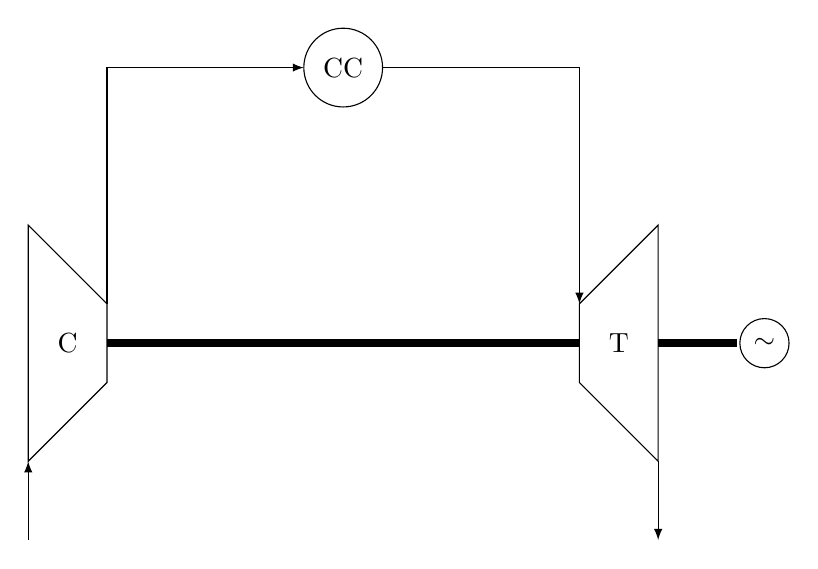
\begin{tikzpicture}[>=latex]
		%\draw [help lines] (0,0) grid (15,15);
		% Compressore
		\draw [->] (2,8) -- (2,9);
		\draw (3,11) -- (2,12) -- (2,9) -- (3,10) -- (3,11) -- cycle;
		% Camera di Combustione e collegamento turbina
		\draw [->] (3,11) -- (3,14) -- (5.5,14);
		\draw (6,14) circle (0.5cm);
		\draw [->] (6.5,14) -- (9,14) -- (9,11);
		\draw [line width=3pt] (3, 10.5) -- (9, 10.5);
		% Turbina
		\draw (9,11) -- (10,12) -- (10,9) -- (9,10) -- (9,11) -- cycle;
		\draw [line width=3pt] (10, 10.5) -- (11, 10.5);
		\node [draw, circle] at (11.35, 10.5) {$\sim$};
		\draw [->] (10,9) -- (10,8);
		% NOMI
		\node at (2.5,10.5) {C};
		\node at (9.5,10.5) {T};
		\node at (6,14) {CC};
	\end{tikzpicture}	
	
	In questa tipologia di impianto si convoglia dell'aria a pressione e temperatura ambiente in un compressore che ha il compito di far aumentare la pressione, dopodiché una camera di combustione aumenta la temperatura ed il fluido caldo viene convogliato in una turbina al fine di estrarre lavoro. 
	
	All'uscita della turbina si avrà un fluido dalle caratteristiche chimiche e fisiche diverse dal fluido in entrata, e a rigore questo non è propriamente un processo ciclico, tuttavia se si assume la presenza di una trasformazione di chiusura che avviene in atmosfera, si può considerare questo sistema come uno \textbf{pseudociclo}. \newline 
	
	Sia per cicli che per psudocicli vale l'assunzione per cui la differenza di energia interna è nulla: se si ritorna periodicamente nelle stesse condizioni, vuol dire che l'energia interna, che è una grandezza di stato e dipende dalle condizioni nel punto isolato, sarà sempre allo stesso valore e la sua differenza nel ciclo sarà nulla. Questo significa che 
	\[L=Q\]
	\textit{Tanto calore immetto, al netto di quello che asporto, tanto lavoro estraggo.} 
	
	Perciò la differenza tra il calore in ingresso $q_1$ e quello in uscita $q_2$ sarà proprio pari a
	\[q_1-q_2=l\]	
	Col secondo principio della termodinamica tuttavia si è introdotto il fatto che le trasformazioni seguono un verso preferenziale, esisteranno allora delle cause di irreversibilità che renderanno una certa trasformazione percorribile in un senso piuttosto che in un altro. 
	
	\newpage
	
	Il caso più comune di irreversibilità è quello relativo agli attriti.  
	
	\vspace{0.5cm}
	
	\begin{tikzpicture}[>=latex]
		\draw (2,1) -- (2,4) --  (3,4) -- (3,3) -- (5,3) -- (5,2) -- (3,2) -- (3,1) -- (2,1) -- cycle;
		\draw [pattern=north east lines] (4.5,2.05) rectangle (5,2.95);
		\draw (4,3.4) -- (4,3.6);
		\draw (4.5,3.4) -- (4.5,3.6);
		\draw (4.5,3.5) -- (4,3.5) node [pos = 0.5, above] {dx}; 
		\draw [->] (4,2.5) -- (3.5,2.5) node [pos=0.5, above] {$F$};
		\draw [->] (3,2.5) -- (3.5,2.5) node [pos=0.5, above] {$F_a$};
		\draw [dashed] (4,2) -- (4,3) node [pos=0.5, right] {$dv$};
		\draw [line width=3pt, ->] (6,2.5) -- (5,2.5) node [pos=0, right] {$l$};
		\draw [line width=3pt, ->] (1.5,2.5) -- (2,2.5) node [pos=0, left] {$q$};
	\end{tikzpicture} 
	
	Si individui una particella di fluido sospinta dal pistone, questa da un lato sarà soggetta ad una forza $F$ di avanzamento ed una forza $F_a$ di attrito, a valle della particella, che si opporrà al moto, purché questo avvenga infatti deve valere $F_a<F$; ciò significa che il lavoro richiesto dalla particella per entrare nel sistema sarà maggiore del semplice termine $P\dfrac{d\rho}{\rho^2}$: il pistone spinge con una certa forza ma al fluido, a causa degli attriti arriva una forza minore, allora si può scrivere 
	\[dl = P\dfrac{d\rho}{\rho^2} + dl_p\]
	Il termine aggiuntivo $dl_p$ (lavoro passivo) esiste sempre nei processi reali, ma si riduce mano a mano che questi vengono realizzati in maniera sempre più lenta, passando per infiniti stati di equilibrio, in questo modo l'azione viscosa di attrito - proporzionale al quadrato della velocità - avrà meno contributo: spingendo il pistone lentamente si avrà meno attrito che spingendo il pistone velocemente; al limite spostando il pistone con una velocità infinitesima, si avranno attriti tendenzialmente nulli. 
	
	Ovviamente i processi reali non avvengono passando per infiniti stati di equilibrio e quindi si registra, oltre che un incremento del lavoro necessario, anche una notevole disomogeneità della pressione: vicino al pistone questa sarà infatti pari a quella esercitata dal pistone stesso, nel punto più remoto del contenitore sarà invece minore. Non esiste puntualmente un valore univoco della pressione, a meno che non si aspetta che il sistema raggiunga l'equilibrio. 
	
	Così come si registrano disomogeneità di pressione, allo stesso modo si registreranno disomogeneità di temperature. \newline
	
	Pressione e temperatura si configurano così come sorgenti irreversibilità di prima specie, quelle di seconda specie sono relative alle trasformazioni chimiche. Ad esempio nella combustione i reagenti producono sempre i prodotti mentre il contrario non è sempre vero, esiste una direzione preferenziale della reazione.\newline
	
	Il concetto di reversibilità consente in questo modo di introdurre una grandezza estremamente importante nei processi termodinamici, l'entropia. 	
	\[du = dq + dl\]
	Ma
	\[dl = P\dfrac{d\rho}{\rho^2} + dl_p\]
	Per cui 
	\[du = dq + P\dfrac{d\rho}{\rho^2} + dl_p \Rightarrow dq + dl_p = du -P\dfrac{d\rho}{\rho^2}\] 
	Entrambi i membri di questa uguaglianza non sono dei differenziali esatti, allora si può sempre scrivere, dividendo per la stessa quantità 
	\[\dfrac{dq + dl_p}{T} = \dfrac{du}{T} -\dfrac{P}{T}\dfrac{d\rho}{\rho^2}\]
	Ovvero, ricordando che $du=c_VdT$ e $P=\rho RT$
	\[\dfrac{dq + dl_p}{T} = c_V\dfrac{dT}{T} -R\dfrac{d\rho}{\rho}\] 
	Il membro di destra ora è costituito da sole grandezze sensibili $T, \rho$, allora è un differenziale esatto, poiché un differenziale esatto può essere uguale solo ad un altro differenziale esatto, allora anche il membro di sinistra è un differenziale esatto e prende il nome di entropia, un'altra grandezza di stato, come $u$ ed $h$:
	\begin{equation}\label{eq:1.11}
		ds = \dfrac{dq}{T} + \dfrac{dl_p}{T}
	\end{equation}
	Si può allora riscrivere il primo principio della termodinamica considerando questa nuova grandezza di stato che porta con se le irreversibilità
	\begin{eqnarray}\label{eq:1.12} \label{eq:1.13}
	\boxed{du = Tds + P\dfrac{d\rho}{\rho^2}}\\
	\boxed{dh = Tds + \dfrac{dP}{\rho}}
	\end{eqnarray}
	L'entropia a seguito dell'adduzione di calore e dell'aumento delle irreversibilità aumenterà sempre. 
	
	L'entalpia invece può tendere a zero solamente nei processi adiabatici dove non si scambia calore, e in special modo nei processi lenti, questi tanto più simili a processi reversibili. 
	
	Già da qui si può osservare una riprova dell'enunciato del secondo principio della termodinamica di Kelvin: è necessaria una fonte di immissione di calore e una fonte di sottrazione del calore per produrre  lavoro continuativo in maniera ciclica. Affinché un sistema sia periodicamente ciclico è necessario tornare sempre ad un certo stato termodinamico, quindi dato che l'entropia è una funzione di stato allora anche questa tornerà la stessa? Se ad esempio si dovesse percorrere l'impianto a vapore precedentemente visto, allora si scoprirà che nella fase iniziale l'entropia aumenta perché si fornisce calore, in seguito nella successiva espansione in turbina, a causa delle irreversibilità intrinseche nel processo, l'entropia continuerà ad aumentare, sarà allora necessario ritornare alle condizioni in ingresso diminuendo l'entropia attraverso una sottrazione di calore,  ecco la necessità di avere due fonti termiche. 
	
	\section{Trasformazioni tecniche dei fluidi}
	
	Tramite l'analisi dei tre principi base della termodinamica sono state introdotte tutte le grandezze  termodinamiche di interesse: quelle sensibili $P,\rho,T$ , e le funzioni di stato  $u, h, s$; ora diviene finalmente possibile analizzare tutte le varie trasformazioni tecniche dei fluidi. \newline 
	
	Alle tre trasformazioni dove le tre rispettive grandezze sensibili si mantengono costanti, se ne aggiunge una quarta
	\begin{itemize}
	\item \textbf{Isocora} a volume costante quindi a densità costante $dv=0$
	\item \textbf{Isobara} a pressione costante $dP=0$
	\item \textbf{Isoterma} a temperatura costante $dT=0$
	\item \textbf{Adiabatica} a calore scambiato nullo, particolarmente significativa perché, dato che si è detto che si scambia O calore O lavoro, l'adiabatica andrà a rappresentare tutti i processi di estrazione del lavoro, come quelli si espansione e di compressione.
	\end{itemize} 
	
	\vspace{0.5cm}
	
	Analizzando un gas perfetto l'energia interna e l'entalpia si configurano essere funzioni solamente della temperatura (in alcuni tipi di gas reali sono funzioni anche della pressione) e allora valendo
	\[\dfrac{P}{\rho} = RT \qquad c_V = \dfrac{du}{dT} \qquad c_p = \dfrac{dh}{dT} \] 
	Si può scrivere 
	\[dh -du = (c_P-c_V)dT\]
	Ricordando la definizione di entalpia ed energia interna
	\[h =  u + \dfrac{P}{\rho}\]
	E quindi 
	\[dh - du = d\left(\dfrac{P}{\rho}\right) = RdT\]
	Da cui è possibile ricavare l'equazione di Mayer
	\begin{equation}\label{eq:1.14}
		\boxed{c_P-c_V = R}
	\end{equation}
	Ricordandosi che
	\[k = \dfrac{c_P}{c_V}\]
	Allora 
	\begin{equation}\label{eq:1.15}
		\boxed{R = c_V(k-1) = c_P\dfrac{k-1}{k} = c_P\varepsilon}
	\end{equation}
	Con $R$ costante specifica del gas ottenuta dividendo quella universale per la massa molare del gas. \newline
	
	Se per un gas perfetto l'energia interna e l'entalpia sono funzione della temperatura, significa che anche il $c_P$ è una funzione della temperatura, e pertanto si può esprimere come una serie polinomiale in cui diversi coefficienti che moltiplicano la temperatura: la formula di Langen (arrestata al primo ordine)	 	  
\begin{equation}\label{eq:1.16}
		\boxed{c_P = a + bT}
\end{equation}
	Il calore specifico misura la variazione di temperatura associata ad una certa quantità di calore, questo significa che al variare della temperatura, la stessa temperatura del fluido si modifica diversamente per il flusso dello stesso calore. Fornire 1 J di calore a 0 \degree C , si comporta un diverso incremento di temperatura, che fornire 1 J di calore a 100 \degree C. 
	
	In una generica trasformazione all'interno della quale si registra una temperatura variabile, a rigore, necessiterà l'utilizzo di questa formulazione di Langen per il calcolo del $c_P$.
	
	Ad esempio una trasformazione di compressione adiabatica ed isoentropica (una linea retta verticale sul piano TS), comporta avere un $c_P$ variabile, per cui o si divide la trasformazione in tantissimi infinitesimali intervalli in cui la differenza di temperatura è limitata ed il $c_P$ diviene costante e poi si sommano tutti i contributi, oppure si considera un $c_P$ medio di trasformazione tra la $T_1$ e $T_2$ e si assumere quel $c_P$ come rappresentativo dell'intera trasformazione. 
	
	Per un gas perfetto (tutti li aeriformi lontano dalle condizioni critiche) il $c_P$ varia solo con la temperatura, se invece sono costanti sia il $c_P$ che il $c_V$ si parla di gas IDEALI. \newline
	
	Adesso diviene allora possibile introdurre l'ultima trasformazione che si può aggiungere alle quattro precedentemente viste, la più generica delle trasformazioni, la \textbf{Politropica}, la trasformazione a calore specifico costante.
	
	Noto che3  
	\[\begin{cases}
		dh = dq + \dfrac{dP}{\rho} \\ du = dq + P\dfrac{d\rho}{\rho^2} 
	\end{cases}\]
	Si può riscrivere come 
	\[\begin{cases}
		c_pdT = cdT + \dfrac{dP}{\rho} \\ c_vdT = cdT + P\dfrac{d\rho}{\rho^2}
	\end{cases}\]
	Dividendo membro a membro
	\begin{equation}\label{eq:1.17}
		\dfrac{c_P-c}{c_V-c} = \dfrac{\dfrac{dP}{P}}{\dfrac{d\rho}{\rho}}=m
	\end{equation}
	Allora 
	\[\dfrac{dP}{P} = m\dfrac{d\rho}{\rho}\]
	Integrando si ottiene 
	\[\ln P = m\cdot\ln\rho + C\]
	E quindi
	\[P = A\cdot\rho^m\]
	Utilizzando l'equazione di stato dei gas perfetti, si può giungere a
	\[T = A'\cdot\rho^{m-1} \qquad T = A''\cdot P^{m-1\over m}\]
	Questa equazione gioca un ruolo fondamentale nel ricavare il lavoro, questo infatti è ricavabile solo se è nota la legge di variazione della pressione con la densità: questa è proprio la funzione che si può integrare per individuare il lavoro. 
	
	Se 1 e 2 sono rispettivamente il punto di inizio e di fine trasformazione, si potrà allora scrivere 
	\[\dfrac{P_2}{P_1} = \left(\dfrac{\rho_2}{\rho_1}\right)^m \qquad \dfrac{T_2}{T_1} = \left(\dfrac{\rho_2}{\rho_1}\right)^{m-1} \qquad \dfrac{T_2}{T_1} = \left(\dfrac{P_2}{P_1}\right)^{m-1\over m}\]
	Si immagini così di avere una trasformazione di compressione e di conoscere sia la pressione in ingresso che quella di uscita, allora è noto il rapporto $\beta={P_2\over P_1}$ e quindi se diviene noto $m$ si può trovare la temperature di fine compressione. \newline
	
	In aggiunta si può trovare il lavoro per sistemi chiusi
	\[\bar{l}_{12} = \int_{1}^{2}P\dfrac{d\rho}{\rho^2} = \dfrac{1}{m-1}\dfrac{P_1}{\rho_1}\left[\left(\dfrac{\rho_2}{\rho_1}\right)^{m-1}-1\right] = \dfrac{1}{m-1}\dfrac{P_1}{\rho_1}\left[\left(\dfrac{P_2}{P_1}\right)^{m-1\over m}-1\right]\]
	E per sistemi aperti
	\[l_{12} = \int_{1}^{2}\dfrac{dP}{\rho} = \dfrac{m}{m-1}\dfrac{P_1}{\rho_1}\left[\left(\dfrac{\rho_2}{\rho_1}\right)^{m-1}-1\right] = \dfrac{m}{m-1}\dfrac{P_1}{\rho_1}\left[\left(\dfrac{P_2}{P_1}\right)^{m-1\over m}-1\right]\]
	La politropica è importante perché è possibile declinarla in diverse trasformazioni.
	\begin{itemize}
		
	\item L'adiabatica è quella trasformazione in cui lo scambio di calore è nullo, allora dalle equazioni viste prima (\ref{eq:1.17}) il coefficiente $c$, calore specifico generico, sarà nullo e quindi 
	\[c=0 \qquad m=k={cp\over cv} \qquad P=A\cdot\rho^k\]
	\[\dfrac{P_2}{P_1} = \left(\dfrac{\rho_2}{\rho_1}\right)^k \qquad \dfrac{T_2}{T_1} = \left(\dfrac{\rho_2}{\rho_1}\right)^{k-1} \qquad \dfrac{T_2}{T_1} = \left(\dfrac{P_2}{P_1}\right)^{k-1\over k}\]
	\item L'isocora 
	\[c=c_V \qquad \rho = cost \qquad \dfrac{P_2}{P_1} = \dfrac{T_2}{T_1}\]
	\item L'isobara 
	\[c=c_P \qquad P = cost \qquad \dfrac{\rho_2}{\rho_1} = \dfrac{T_1}{T_2}\]
	\item L'isoterma 
	\[c=\infty  \qquad T = cost \qquad P=A\cdot\rho \qquad \dfrac{P_2}{P_1} = \dfrac{\rho_2}{\rho_1}\]
	\end{itemize}	 
	
	\section{Piani di rappresentazione}
	Se si inseriscono sui due assi di un piano cartesiano due variabili di stato, si otterrà una descrizione completa dello stato fisico di un solo punto, infatti essendo la varianza al massimo pari a due, i due assi corrispondono esattamente ai due membri della varianza: per ogni coordinata si descrive in maniera completa lo stato fisico del sistema. 
	
	A rigore sarebbe possibile rappresentare solo le trasformazioni reversibili, perché se si afferma che un punto rappresenta completamente il sistema, significa che nel sistema le grandezze sono completamente omogenee, non ci sono discrepanze, ma a causa di attriti ed irreversibilità ci saranno sempre delle variazioni all'interno del sistema: la rappresentazione sui piani termodinamici funziona solamente se si effettuano delle trasformazioni talmente lente che la variabilità delle grandezze sensibili all'interno del dominio risulta estremamente limitata.
	
	In sostanza, per rappresentare delle trasformazioni reali si utilizzeranno delle politopiche passanti per i punti estremali delle trasformazioni reali. 
	
	Il primo piano che si analizza è quello $Pv$, pressione-volume specifico.
	
		\scalebox{0.6}{\begin{tikzpicture}[>=latex,
		dot/.style = {draw,fill,circle,inner sep=1pt},arrow inside/.style = {postaction=decorate,decoration={markings,mark=at position .55 with \arrow{>}}}]
		%\draw [help lines] (0,0) grid (10,10);		
		\draw[->] (0,0) -- (10,0) node [pos=1, right] {$P$};
		\draw[->] (0,0) -- (0,10) node [pos=1, above] {$v$};
		%ISOBARA
		\node[dot] (@P1) at (4,9) {};
		\node[dot] (@P2) at (9,9) {};
		\draw(@P1) -- (@P2) node [pos = 0.5, above] {isobara};
		%ISOCORA
		\node[dot] (@V1) at (8,7) {};
		\node[dot] (@V2) at (8,3) {};
		\draw(@V1) -- (@V2) node [pos = 0.5, sloped, above] {isocora};
		%ADIABATICA
		\node[dot] (@Q1) at (1,8) {};
		\node[dot] (@Q2) at (3,1) {};
		\draw [looseness=.4,bend right=20,postaction={decorate,
			decoration={text along path, text align={center}, text={adiabatica}, raise=5pt}}] (@Q1) to  (@Q2);
		%ISOTERMA
		\node[dot] (@T1) at (2,8) {};
		\node[dot] (@T2) at (8,1) {};
		\draw [looseness=1,bend right=20, postaction={decorate,
			decoration={text along path, text align={center}, text={isoterma}, raise=5pt}}] (@T1) to  (@T2);									
	\end{tikzpicture}}
	
	L'isoterma è più pendente perché avrà un'equazione del tipo $Pv=cost$ e quindi è un'iperbole, invece l'adiabatica avrà  un'equazione del tipo $Pv^k = cost$ e quindi sarà una curva esponenziale. 
	
	Sul  piano $Pv$, l'area sottesa rispetto all'asse $x$ rappresenta il lavoro per sistemi chiusi $\bar{l}$, mentre l'area sottesa rispetto all'asse $y$, quello per sistemi aperti. 
	
	Questo piano termodinamico rimane tuttavia poco utilizzato perché prima di tutto non permette di visualizzare gli scambi di calore, e poi perché, soprattutto nei sistemi in cui è presente il passaggio di fase acqua-vapore, dato che il volume specifico ha una variazione molto significativa, questa rappresentazione non permette un'agevole visualizzazione d'impatto delle trasformazioni.\newline 
	
	Un altro piano molto utilizzato è il piano $Ts$, temperatura - entropia 
	
	p.319 fig17
	
	L'isocora è più inclinata dell'isobara perché essendo 
	\[ds = \dfrac{dq}{T} =  \dfrac{cdT}{T}\]
	Integrando 
	\[\Delta s = c\ln\dfrac{T_2}{T_1} \]	
	Prendendo un punto P e tracciandone la tangente si possono individuare l'angolo $\alpha$, l'arco sotteso $s$ e la grandezza verticale T
	
	p.320 fig18		
	
	Per cui  
	\[s = \dfrac{T}{\tan\alpha} \] 
	Ma 
	\[\dfrac{T}{\tan\alpha} = \dfrac{dT}{ds} \]	
	E quindi 
	\[s = \dfrac{T}{\dfrac{dT}{ds}} = \dfrac{Tds}{dT} = \dfrac{dq}{dT} = c \] 
	L'arco sotteso al punto tangente alla curva  corrisponde al calore specifico, dato che il calore specifico a pressione costante è maggiore di quello a volume costante, si ottiene che l'arco $s$ sotteso all'isobara è maggiore e la curva risulta meno inclinata, viceversa per l'isocora.\newline
	
	La caratteristica più importante del piano $Ts$, è che se si effettua l'integrale 
	\[\int Tds =q + l_p\]
	L'area sottesa alle trasformazioni rappresenta: il calore per trasformazioni ideali, e per quelle reali il calore più il contributo delle forze d'attrito. \newline
	
	Inoltre per dei gas perfetti o comunque per quelli i quali la variazioni di $c_P$  è limitata con la temperatura, il diagramma $Ts$ ed il diagramma $hs$ coincidono a meno di un fattore di scala, d'altronde 
	\[dh = c_PdT\]
	Se in un grafico $Ts$ si moltiplicano tutti i valori di $T$ per $c_P$, questo diventa un grafico $hs$: per i gas il grafico $Ts$ ha doppia valenza (aggiungi h alla figura). \newline
	
	Il diagramma $hs$ è interessante  perché è noto che 
	\[dh = dq + dl\]
	In più si è visto che le trasformazioni o producono calore o producono lavoro, quindi a partire da un diagramma $hs$, attraverso la differenza di coordinata $h$  diviene  possibile calcolare la differenza di entalpia di ogni trasformazione, che saranno riconducibili o a scambi si calore o a scambi di lavoro a seconda della trasformazione. \newline
	
	
	Infine  si fa notare che in un diagramma $Ts$, se il gas è perfetto, essendo il $c_P$ la tangente della curva, non varia con la pressione, ma solo con la temperatura, quindi una curva a pressione diversa avrà la stessa identica forma ma sarà solamente traslata orizzontalmente verso la pressione più bassa (le isobare divergono nei piani $Ts$ ed $hs$).
	
	Questo fatto è importante perché si nota che le differenza di pressione a temperature via via maggiori geometricamente aumenta, e deriva proprio dal fatto che questa è una curva traslata: ciò significa che, la differenza di entalpia che si ottiene espandendo a temperature elevata  è maggiore della differenza di entalpia che è richiesta comprimendo a minor temperatura: le isobare sono divergenti.
	Ciò è estremamente importante perché - ad esempio - affinché un gruppo turbogas sia effettivamente produttivo, è necessario che  il lavoro prodotto nella turbina, quindi espandendo ad alta temperatura, sia maggiore del lavoro richiesto dal compressione, altrimenti non avviene produzione. 
	
	
\end{adjustwidth}
\newpage
\section{Sistemi acqua - vapore}
\begin{adjustwidth}{2in}{}
	È ora noto che i piani $Ts$ ed $hs$ per i gas assumono la stessa forma, questo perché il fattore di conversione risulta essere solamente il calore specifico che in molti casi può essere assunto indipendente dalla pressione. \newline
	
	Tuttavia nel caso dei sistemi acqua vapore, nel range di temperature di normale impiego nei sistemi energetici ci si trova in prossimità delle condizioni critiche, questo non permette di utilizzare l'ipotesi di gas perfetto, ci si avvarrà perciò per la caratterizzazione degli stati termodinamici delle tabelle del vapore.
	
	Questa caratteristica in più rende i diagrammi $Ts$ ed $hs$ totalmente differenti tra loro, diversamente a quanto fatto per i gas. 
	
	Nello specifico:
	
	GENERICO DISEGNO DEL PIANO TS
	
	GENERICO DISEGNO DEL PIANO HS 
\end{adjustwidth}
\newpage
\section{Trasformazione di compressione}
\begin{adjustwidth}{2in}{}



	
	In che modo effettuare una trasformazione di compressione da $P_1$ a $P_2$? \newline 
	\begin{itemize}
		
		\item Attraverso l'isoterma $1-2'$ 
		
		Non è fattibile, in compressione la temperatura aumenta, questo significherebbe dover continuare a raffreddare il fluido per mantenere la temperatura costante.
		
		Tuttavia, è l'unica trasformazione a richiedere il minimo lavoro in virtù del fatto che la densità è maggiore 
		\[dl = {dP\over\rho}\Rightarrow l_t=RT_1\ln\left(P_2\over P_1\right)\]
		Inoltre, poiché $\Delta h = 0$, vale l'equivalenza 
		\[q=l=A_{A12"C}\]
		
		\item Attraverso l'adiabatica ideale $1-2$
		
		L'adiabatica ideale (isoentropica) è caratterizzata da $dQ =0$, allora varrà 
		\[dl_{is} = dh = c_PdT \Rightarrow l = \int c_PdT = \dfrac{k}{k-1} {P_1\over\rho_1}\left[\left(P_2\over P_1\right)^{\dfrac{k-1}{k}}-1\right]\]
		Il lavoro è misurato dal calore che si scambierebbe lungo una qualsiasi isobara, tra le temperature di riferimento. 
		
		\textbf{NB} $h_1 = h_{2"}~$: tutti i punti alla stessa temperatura hanno la stessa entalpia, d'altro canto questa è una variabile di stati, allora si può scrivere 
		\[l = h_2-h_1 = h_2 -  h_{2"} = A_{A22"C}\]
		
		
		
		\item Attraverso l'adiabatica reale $1-2'$
		
		L'adiabatica reale si sviluppa ad entropie crescenti rispetto ad un'adiabatica ideale e può essere rappresentata attraverso una politropica equivalente con esponente $m>k$, che leghi gli stati 1 e 2' secondo la relazione  
		\[\left(P_2\over P_1\right)^{\dfrac{m-1}{m}} = {T_{2'}\over T_1}\] 
		E allora il lavoro reale si può scrivere come 
		\[\begin{split}
			l_r = \int_{1}^{2'}c_PdT = c_P(T_{2'}-T_1) = c_PT_1\left[\left(P_2\over P_1\right)^{\dfrac{m-1}{m}}-1\right]= \\ \dfrac{k}{k-1} {P_1\over\rho_1}\left[\left(P_2\over P_1\right)^{\dfrac{m-1}{m}}-1\right] = A_{B2'2"C}
		\end{split}\]
		Il lavoro politropico parimenti è  
		\[l_\text{pol} =  \dfrac{m}{m-1} {P_1\over\rho_1}\left[\left(P_2\over P_1\right)^{\dfrac{m-1}{m}}-1\right]= A_{A12'2"C}\]
	\end{itemize}
	
	
	La differenza tra il lavoro isoentropico e quello reale è data da due contributi:
	
	\begin{enumerate}
		\item Il lavoro passivo, perso a cause delle forze d'attrito
		\[A_{A12'B} = l_p\]
		\item Il lavoro di controrecupero, dovuto al fatto che il gas che viene compresso ha una temperatura superiore (e quindi una densità inferiore) rispetto a quella che avrebbe avuto in una compressione isoentropica. 
		\[A_{12'2} = l_{cr}\]			
		Infatti
		\[\begin{matrix}
			\text{Processo Isoentropico}\qquad l_{is} = \int_{1}^{2}dh_{is} = \cancel{\int_{1}^{2}T_0ds} + \int_{1}^{2} {dP_0\over\rho_0} \\
			\text{Processo reale}\qquad l_r = \int_{1}^{2'}dh_0 = \int_{1}^{2'}T_0ds + \int_{1}^{2'} {dP_0\over\rho_0} \\
		\end{matrix}\]
		Allora 
		\[l_r - l_{is} = \underbrace{\int_{1}^{2'}T_0ds}_\text{Lavoro Perso $l_p$} + \underbrace{\int_{1}^{2'} {dP_0\over\rho_0} - \int_{1}^{2} {dP_0\over\rho_0}}_\text{Lavoro di Controrecupero $l_{cr}$}\]
		Il lavoro di controrecupero è dovuto non alle perdite, ma piuttosto alla minore densità del fluido durante la compressione reale. 
	\end{enumerate}
	
	In formule, il lavoro di controrecupero si può scrivere, dal diagramma
	\[l_{cr} = A_{A22'B} - A_{A12'B} = \Delta l - l_p\]
	Per cui
	\[\Delta l = l_r-l_{is} = A_{B2'2"C} - A_{A22"C} = \dfrac{k}{k-1}{P_1\over\rho_1}\left[\left(P_2\over P_1\right)^{\dfrac{m-1}{m}}-\left(P_2\over P_1\right)^{\dfrac{k-1}{k}}\right]\]
	Mentre
	\[l_p = A_{B2'2"C} - A_{A12'2"C} =  l_r - l_{pol} = \left(\dfrac{k}{k-1}-\dfrac{m}{m-1}\right){P_1\over\rho_1}\left[\left(P_2\over P_1\right)^{\dfrac{m-1}{m}}-1\right]\]
	Per cui
	\[l_{cr} = {P_1\over\rho1}\left\{\dfrac{k}{k-1}\left[1-\left(P_2\over P_1\right)^{\dfrac{k-1}{k}}  \right] - \dfrac{m}{m-1}\left[1+\left(P_2\over P_1\right)^{\dfrac{m-1}{m}}  \right] \right\}\] 
	La bontà di un compressore verrà indicata dal parametro $\eta$
	\[\eta = {l_\text{rev}\over l_\text{real}}<1\]
	\begin{itemize}
		\item Il rendimento isotermo sarà il minore di tutti
		\[\eta_T = {l_T\over l_r}\]
		E si terrà in considerazione per compressori polistadio con interrefrigerazioni.
		\item Il rendimento isoentropico (o adiabatico) viene utilizzato per l'analisi di massima del sistema energetico, è in questa fase che entra in gioco il lavoro di controrecupero.
		\[\eta_{is} = {l_{is}\over l_r}\]
		\item Il rendimento politropico viene usato per sviluppare il compressore e quantifica l'effetto del lavoro delle forze d'attrito, in questa fase NON entra in gioco il lavoro di controrecupero, questo infatti non dipende dal compressore
		\[\eta_{pol} = {l_\text{pol}\over l_r}\]
		
		\[\eta_{pol} = \dfrac{\dfrac{m}{m-1} \dfrac{P_1}{\rho_1}\left[\left(\dfrac{P_2}{P_1}\right)^{\dfrac{m-1}{m}}-1\right]}{\dfrac{k}{k-1}\dfrac{P_1}{\rho_1}\left[\left(\dfrac{P_2}{P_1}\right)^{\dfrac{m-1}{m}}-1\right]} = \dfrac{m}{m-1}\cdot\dfrac{k-1}{k}\]
		Si può perciò conoscere l'esponente della politropica a partire dal rendimento politropico, infatti
		\[\dfrac{m-1}{m}= \dfrac{1}{\eta_{pol}}\dfrac{k-1}{k}\]
		E quindi
		\[\dfrac{T_{2'}}{T_1} = \beta^{\dfrac{m-1}{m}} = \beta^{ \dfrac{1}{\eta_{pol}}\dfrac{k-1}{k}}\]
		Si può calcolare la $T_{2'}$ di fine compressione reale conoscendo $\eta$ e $k$. 
	\end{itemize}
	Vale sempre 
	\[\eta_T<\eta_{is}<\eta_\text{pol}\]
\end{adjustwidth}




\section{Trasformazione di espansione}
\begin{adjustwidth}{2in}{}
	DISEGNO fatto bene
	
	Similmente a quanto visto per la compressione, con la trasformazione di espansione si può produrre lavoro attraverso
	\begin{itemize}
		\item L'isoterma $1-2"$
		\[l = A_{A12"C}\]
		\item L'adiabatica isoentropica $1-2$\\
		Poiché il lavoro si può rappresentare come calore scambiato a pressione costante, ad esempio a $P_2$, si può scrivere
		\[l_{is} = \int_{2}^{1} \dfrac{dP_0}{\rho_0} \dfrac{k}{k-1}\dfrac{P_1}{\rho_1}\left[1-\left(\dfrac{P_2}{P_1}\right)^{\dfrac{k-1}{k}}\right] = A_{A22"C}\]
		Notare inoltre come 1 si trovi alla stessa temperatura di 2.
		\item L'adiabatica reale 
		\[l_r = \int_{2'}^{1}T_0ds + \int_{2}^{1}\dfrac{dP_0}{\rho_0} \dfrac{k}{k-1}\dfrac{P_1}{\rho_1}\left[1-\left(\dfrac{P_2}{P_1}\right)^{\dfrac{m-1}{m}}\right] = A_{B2'2"C}\]
		A cui è associata il lavoro della politropica 
		\[l_{pol} = \dfrac{m}{m-1}\dfrac{P_1}{\rho_1}\left[1-\left(\dfrac{P_2}{P_1}\right)^{\dfrac{m-1}{m}}\right] = A_{A12'B}\]
	\end{itemize}
	Anche in questo caso la differenza tra il lavoro isoentropico e quello reale è data da due contributi:
	
	\begin{enumerate}
		\item Il lavoro passivo, perso a cause delle forze d'attrito
		\[A_{A12'B} = l_p\]
		\item Il lavoro di recupero, dovuto al fatto che il gas viene espanso dal calore prodotto dall'attrito 
		\[A_{212'} = l_R\]			
		Infatti
		\[\begin{matrix}
			\text{Processo Isoentropico}\qquad l_{is} = -\int_{1}^{2}dh_{is} = \cancel{-\int_{1}^{2}T_0ds}  -\int_{1}^{2} {dP_0\over\rho_0} \\
			\text{Processo reale}\qquad l_r = -\int_{1}^{2'}dh_0 = -\int_{1}^{2'}T_0ds - \int_{1}^{2'} {dP_0\over\rho_0} \\
		\end{matrix}\]
		Allora 
		\[l_{is} - l_r = -\int_{1}^{2} {dP_0\over\rho_0} - \left[-\int_{1}^{2'}T_0ds - \int_{1}^{2'} {dP_0\over\rho_0}\right] = \]
		\[ = \underbrace{-\int_{2'}^{1}T_0ds}_\text{Lavoro Perso $l_p>0$} + \underbrace{\int_{2}^{1} {dP_0\over\rho_0} - \int_{2'}^{1} {dP_0\over\rho_0}}_\text{Lavoro di Recupero $l_R<0$}\]
		Il lavoro di recupero
		\[\int_{2'}^{1} {dP_0\over\rho_0} - \int_{2}^{1} {dP_0\over\rho_0}>0\] 
		È positivo per il fatto che la densità nell'espansione reale è minore che in quella ideale  
	\end{enumerate}
	In formule il lavoro di recupero può essere individuato dal diagramma come 
	\[l_R = A_{A12'B} - A_{A22'B} =  l_\text{pol} - |\Delta l| \]
	\[|\Delta l| = |l_r-l_{is}| = A_{B2'2"C} - A_{A22"C} = A_{A22'B} = \dfrac{k}{k-1}\dfrac{P_1}{\rho_1}\left[\left(\dfrac{P_2}{P_1}\right)^{\dfrac{m-1}{m}} - \left(\dfrac{P_2}{P_1}\right)^{\dfrac{k-1}{k}}\right]\]
	Si nota subito come questo contributo risulti minore dell'area sottesa alla politropica equivalente, questa misura il lavoro delle forze d'attrito $l_{pol} = A_{A12'B}$. 
	
	Si ricava allora che nell'espansione adiabatica la perdita di lavoro a causa degli attriti è inferiore al lavoro d'attrito (identificato dalla politropica), ciò vuol dire che una parte del lavoro d'attrito viene recuperata: la differenza tra il lavoro politropico e il contributo $|\Delta l|$ porta ad identificare il lavoro di recupero $l_R$
	\[l_{pol} - |\Delta l| = A_{A12'B} - A_{A22'B} = A_{212'} = l_R\]
	Il lavoro di recupero agisce questa volta "positivamente". Infatti il gas, sempre a causa dell'attrito, ha una temperatura maggiore (e quindi una densità minore) di quella che avrebbe avuto in un processo di espansione senza perdite, viene dilatato "gratuitamente" e quindi permette di produrre più lavoro. 
\end{adjustwidth}




\section{Processi Ciclici}
\begin{adjustwidth}{2in}{}
	Un ciclo termodinamico è una catena chiusa di trasformazioni. 
	
	In uno pseudociclo termodinamico la catena di trasformazioni è aperta (macchine a combustione interna): una reazione chimica trasforma le proprietà del fluido, il ciclo inizia con un fluido e termina coi prodotti della combustione. \newline 
	
	Si possono tuttavia considerare gli pseudocicli termodinamici come veri e propri cicli, nei quali si ipotizza una trasformazione di chiusura che provveda a ristabilire  le condizioni iniziali del fluido. \newline 
	
	Il ciclo di Carnot è l'unico ciclo che massimizza il rendimento termodinamico operando tra due sole sorgenti termiche, è un ciclo ideale. 
	
	Un ciclo reale opera tra "infinite" sorgenti termiche. 
	
	DISEGNO dei due cicli 	
\end{adjustwidth}




\subsection{Equivalenza tra i principi di Kelvin e Clausius} \label{par:eq}
\begin{adjustwidth}{2in}{}
	DISEGNO
	
	Si ponga un corpo caratterizzato da $T_0, S_0$ a contatto con un altro corpo caratterizzato dalla stessa capacità termica avente $T_A, S_A$; ad un certo istante di tempo raggiungeranno la temperatura di equilibrio $T_B = {T_A\over2}$, il calore scambiato durante la trasformazione sarà l'area sottesa alla stessa $\int dT = Q$, che non deve e non può cambiare, allora $S_B>S_A$: per produrre lavoro si dovrà apportare calore ma si aumenta l'entropia: per poter estrarre ciclicamente lavoro sarà allora necessario fornire calore, ma per far avvenire il processo ciclico, dovrà avvenire un raffreddamento che riporti il fluido alle condizioni di entropia iniziali, d'altronde in un ciclo
	\[\Delta u = \Delta h = \Delta s = 0\Rightarrow L = Q_1-Q_2 \Rightarrow \underline{W} = \dot{m}l\]
	Se si vuole massimizzare la potenza estratta dal ciclo si può agire accrescendo la portata, e quindi ottenendo una macchina più grande, a parità di macchina si opera in modo da aumentare $Q_1$, il calore fornito al ciclo, e ridurre $Q_2$ il calore ceduto dal ciclo, in sostanza si opera per ridurre il coefficiente $\theta={Q_2\over Q_1}$, la frazione di calore non utilizzato, d'altro canto è possibile mettere in relazione questa quantità col rendimento
	\[\eta = 1 - \theta\]
	Diventa così visibile il fatto che una diminuzione di $\theta$ comporta un aumento di $\eta$.  
\end{adjustwidth}




\subsection{Rappresentazione dei cicli}
\begin{adjustwidth}{2in}{}
	Una sequenza di trasformazioni termodinamiche può essere rappresentato secondo un ciclo 
	\begin{itemize}
		\item \textbf{Ideale}\\
		Dove si considera il fluido ideale e quindi come un gas perfetto dalle $c_P, c_V$ costanti con la temperatura e si utilizzano macchine perfette senza perdite. \newline 
		
		Per un ciclo turbina a gas si può scrivere 
		
		DISEGNO
		\[T_1, P_1\rightarrow\text{Note}; \quad T_2 = T_1\beta^{k-1\over k}; \quad T_3 \rightarrow\text{Imposta da limiti tecnologici} \quad T_4 = \dfrac{T_3}{\beta^{k-1\over k}}\]		
		\[P_2 = \beta P_1; \qquad P_2=P_3; \qquad P_4 = P_1; \qquad k=1.4\]		
		\[\rho_1 = \dfrac{P_1}{RT_1}; \quad \rho_2 = \rho_1\beta^{1\over k}; \qquad \rho_3 = \dfrac{P_3}{RT_3}; \qquad \rho_4 = \dfrac{P_4}{RT_4}\]
		Per cui
		\[Q_1^\text{id} = c_P(T_3-T_2)\qquad Q_2^\text{id} = c_P(T_4-T_1)\]
		Se $\varepsilon = \dfrac{k-1}{k}$  E 
		$\tau = \dfrac{T_3}{T_1}$ si può scrivere il lavoro del ciclo ideale come
		\[|L_{id}| = Q_1^\text{id} - Q_2^\text{id} = c_P(T_3-T_2-T_4+T_1) = c_PT_1\left[\tau\left(1-\dfrac{1}{\beta^\varepsilon}\right)+1 -\beta^\varepsilon\right]\]
		Ed il rendimento come 
		\[\eta = \dfrac{|L_{id}|}{Q_1} = 1-\dfrac{Q_2^\text{id}}{Q_1^\text{id}} = 1 - \dfrac{T_4-T_1}{T_3-T_2} = 1 - \dfrac{1}{\beta^\varepsilon}\]
		Il ciclo ideale porta a risultati molto approssimati, e scarsamente significativi.
		\item \textbf{Limite}\\
		Il fluido diviene reale, $c_P, c_V = f(T)$ e si continuano a considerare le macchine perfette, per individuare le caratteristiche termofisiche del fluido si utilizzano le tabelle del vapore e si effettuano iterazioni numeriche per individuare il giusto coefficiente in funzione della temperatura fornita. \newline 
		
		Il ciclo limite, per antonomasia, è il limite massimo a cui può tendere un ciclo perfezionando la macchina. 
		\item \textbf{Reale}\\
		Il fluido è reale e la macchina è reale, entrano in gioco gli attriti. 
		
		DISEGNO CICLO REALE
	\end{itemize}
	Vale sempre 
	\[\eta_R<\eta_L<\eta_I\]
\end{adjustwidth}




\subsection{Criteri di valutazione del rendimento}
\begin{adjustwidth}{2in}{}
	Il rendimento di un ciclo termodinamico può essere valutato attraverso 
	\begin{itemize}
		\item l'effetto Carnot
		\item l'effetto di molteplicità delle sorgenti 
		\item l'Effetto Clausius
	\end{itemize}
\end{adjustwidth}





\subsubsection{Effetto Carnot}
\begin{adjustwidth}{2in}{}
	\begin{en}
		Fissate due temperature estreme, il ciclo di massimo rendimento evolvente tra tali temperature, è il ciclo di Carnot. 
		
		Un qualsiasi ciclo termodinamico ha rendimento inferiore a quello del ciclo di Carnot evolvente tra le medesime temperature estreme.
	\end{en}
	
	Grafico
	
	\begin{proof}
		Per un ciclo di Carnot i rapporti manometrici di compressione e di espansione adiabatica sono pari a
		\[\dfrac{P_2}{P_1} = \dfrac{P_3}{P_4} = \left(\dfrac{T"}{T'}\right)^{k-1\over k}\]
		Si può quindi scrivere 
		\[\dfrac{P_3}{P_2} = \dfrac{P_4}{P_1}\]
		Il calore fornito e ceduto assumono rispettivamente la forma 
		\[Q_1^* = RT"\ln\left(\dfrac{P_3}{P_2}\right) \qquad Q_2^* = RT'\ln\left(\dfrac{P_4}{P_1}\right)\]
		E il rendimento si può così scrivere 
		\[\eta^* = 1-\dfrac{Q_2^*}{Q_1^*} = 1- \dfrac{T'}{T"}\]
		Per cui all'aumentare di $T"$ aumenterà anche il rendimento.\newline 
		
		Si consideri adesso un ciclo generico operante tra gli stessi valori massimi di quello di Carnot, ovvero che sia compreso al suo interno, varrà giocoforza 
		\[Q_1<Q_1^* \qquad Q_2>Q_2^*\]
		Allora 
		\[\eta = 1-\dfrac{Q_2}{Q_1} < 1-\dfrac{Q_2^*}{Q_1^*} = \eta^*\]
	\end{proof}	
\end{adjustwidth}




\subsubsection{Effetto di Molteplicità delle Sorgenti}
\begin{adjustwidth}{2in}{}
	\begin{en}(1)
		Il rendimento di un ciclo è la media pesata dei rendimenti dei cicli parziali, presi i caliri assorbiti dal fluido nel corso dei medesimi
	\end{en}
	
	\begin{proof}
		Un qualsiasi ciclo termodinamico può essere suddiviso in un qualsivoglia numero di sottocicli mediante virtuali trasformazioni isoentropiche. 
		
		disegno
		
		\[L_\text{tot} = L_I + L_{II} + L_{III}\qquad Q_{1,\text{tot}} = Q_{1,I} + Q_{1,II} + Q_{1,III}\]
		Allora 
		\[\eta_I = \dfrac{L_I}{ Q_{1,I}} \qquad \eta_{II} = \dfrac{L_II}{ Q_{1,II}} \qquad \eta_{III} = \dfrac{L_{III}}{ Q_{1,III}}\]
		E quindi
		\[\eta=\dfrac{L}{Q_1} = \dfrac{\eta_{I} Q_{1,I} + \eta_{II} Q_{1,II} + \eta_{III} Q_{1,III} }{Q_{1,II} + Q_{1,II} + Q_{1,III}} = \dfrac{\sum_i\eta_iQ_{1,i}}{\sum_iQ_i}\]
	\end{proof}
	\begin{en}(2)
		In un ciclo che presenti molteplicità di sorgenti, il rendimento tanto più si allontana da quello di Carnot quanto maggiore è l'escursione di temperatura che interessa gli scambi di calore.
	\end{en} 
	
	\begin{proof}
		E se le suddivisioni del ciclo fossero infinite? 
		
		Per ciascun ciclo parziale infinitesimo si possono individuare due e due sole temperature di esercizio, questo vuol dire che si può confondere con un ciclo di Carnot, allora si può scrivere, per l'effetto di molteplicità suddetto
		\[\eta=\dfrac{\int_{A}^{B}\eta^*dQ_1}{\int_{A}^{B}dQ_1} = \dfrac{\int_{A}^{B}\left(1 - \dfrac{T'}{T"}\right)dQ_1}{\int_{A}^{B}dQ_1} = 1 - \dfrac{\int_{A}^{B}\dfrac{T'}{T"}}{\int_{A}^{B}dQ_1}\]
		Per il teorema della media, esiste sempre nell'intervallo $A-B$ un valore di temperatura $T'_m$ compreso tra $T'_{\min}$ e $T'_{\max}$, cosi come esiste sempre un valore di temperatura $T"_m$ compreso tra $T"_{\min}$ e $T"_{\max}$, quindi si può scrivere 
		\[\eta=1-\dfrac{T'_m}{T''_m}\dfrac{\int_{A}^{B}dQ_1}{\int_{A}^{B}dQ_1} = 1-\dfrac{T'_m}{T''_m}\]
		Poiché $T'_m>T'_{\min}$ e $T''_m<T''_{\max}$ allora i coefficienti
		\[\xi'=\dfrac{T'_m}{T'_{\min}}>1\qquad \xi''=\dfrac{T''_m}{T''_{\max}}<1 \qquad\Rightarrow \xi = \dfrac{\xi'}{\xi''}>1\]
		La quantità $\xi$ definita come grado di irreversibilità, dà informazioni su quanto il rendimento si discosta dall'unità. 
	\end{proof}
	\[\eta_{generico} = 1-\xi\dfrac{T'_{\min}}{T''_{\max}}<\eta^*\]
	In sostanza l'effetto di molteplicità delle sorgenti sancisce che, il ciclo si discosta dall'idealità, e quindi da quello di Carnot, quanto più è elevata la gamma di temperature alla quale avvengono gli scambi termici. \newline
	
	Per un ciclo turbogas, infatti 
	
	DISEGNO CICLO fig 40 p353
	
	La temperatura di fine espansione $T_4$ è maggiore della temperatura di inizio combustione $T_2$, si usa allora rigenerare una parte di calore in uscita per effettuare la prima parte di riscaldamento. 
	
	DISEGNO IMPIANTO
	
	Attraverso la rigenerazione diminuisce la gamma di temperature alla quale si scambia calore e si riduce così l'effetto di molteplicità delle sorgenti.
	
	
	
\end{adjustwidth}





\subsubsection{Effetto Clausius}
\begin{adjustwidth}{2in}{}
	L'effetto Clausius tiene conto delle irreversibilità.
	
	disegno fig41 p354
	
	Infatti per una generica trasformazione si avrà inevitabilmente una generazione di entropia 
	\[\Delta s = s_A-s_B\]
	Essendo 
	\[\eta = 1-\dfrac{q_2}{q_1}\]
	E poiché 
	\[Q = \int Tds = T_m\underbrace{sds}_{\sigma} = T_m\sigma\]
	Dove $\sigma$ rappresenta la generica generazione di entropia, allora si può scrivere 
	\[\eta = 1-\dfrac{T'_m\sigma'}{T''_m\sigma''} = 1-\sigma\dfrac{T'_m}{T''_m}\]
	Applicando l'effetto di molteplicità delle sorgenti si perviene a
	\[\eta =1-\sigma\xi\dfrac{T'_{\min}}{T''_{\max}}<\eta^*\]
	Col risultato che più fattori di irreversibilità vengono introdotti e più $\sigma$ cresce, comportando un rendimento minore: $\sigma$ misura l'irreversibilità del ciclo. \newline 
	
	Attraverso quest'ultima relazione si può scrivere
	\[\begin{aligned}
		\begin{cases}
			\eta =1-\sigma\xi\dfrac{T'_{\min}}{T''_{\max}} \Rightarrow \dfrac{T'_{\min}}{T''_{\max}}  = \dfrac{1}{\sigma\xi}(-\eta+1)\\
			\eta^*  =1-\dfrac{T'_{\min}}{T''_{\max}} \Rightarrow \dfrac{T'_{\min}}{T''_{\max}}  = -\eta^*+1
		\end{cases}
	\end{aligned}\]
	Uguagliando i rapporti di temperatura si ottiene 
	\[\dfrac{1}{\sigma\xi}(-\eta+1) = -\eta^*+1\]
	E quindi
	\[\underbrace{1-\eta}_{\theta} = \sigma\xi\underbrace{(1-\eta^*)}_{\theta^*}\]
	In cui si individuano i coefficienti $\theta$ e $\theta^*$ che rappresentano rispettivamente la frazione di calore non utilizzata nel ciclo generico e in quello di Carnot operante tra le stesse temperature massima e minima di quello generico, per cui
	\[\dfrac{\theta}{\theta^*}=\sigma\xi\]
	Poiché l'obbiettivo è quello di minimizzare la frazione di calore non utilizzata, si dovrà necessariamente minimizzare contemporaneamente sia l'effetto Clausius $(\sigma)$ che quello di molteplicità delle sorgenti $(\xi)$. \newline 
	
	Si noti che la rigenerazione termica, come visto, riduce il fattore $\xi$, ma introduce altresì uno scambio di calore intrinsecamente irreversibile, comportando un aumento di $\sigma$.
\end{adjustwidth}